%%%%%%%%%%%%%%%%%%%%%%%%%%%%%%%%%%%%%%%%%%%%%%%%%%%
%% LaTeX book template                           %%
%% Author:  Amber Jain (http://amberj.devio.us/) %%
%% License: ISC license                          %%
%%%%%%%%%%%%%%%%%%%%%%%%%%%%%%%%%%%%%%%%%%%%%%%%%%%

\documentclass[a4paper,11pt]{book}
\usepackage[T1]{fontenc}
\usepackage[utf8]{inputenc}
\usepackage{lmodern}
%%%%%%%%%%%%%%%%%%%%%%%%%%%%%%%%%%%%%%%%%%%%%%%%%%%%%%%%%
% Source: http://en.wikibooks.org/wiki/LaTeX/Hyperlinks %
%%%%%%%%%%%%%%%%%%%%%%%%%%%%%%%%%%%%%%%%%%%%%%%%%%%%%%%%%
\usepackage{hyperref}
\usepackage{graphicx}
\usepackage[english]{babel}
\usepackage[a4paper,top=2cm,bottom=2cm,left=2cm,right=2cm]{geometry}
\usepackage{lscape}
\usepackage{caption}
\usepackage{amsmath}
\usepackage{listingsutf8}

\usepackage{wrapfig}
\usepackage{rotating}
\usepackage{epstopdf}

\usepackage[ruled]{algorithm2e}
\lstset{% general command to set parameter(s)
	basicstyle=\small, % print whole listing small
	numbers=left,
	keywordstyle=\color{black}\bfseries,
	% underlined bold black keywords
	identifierstyle=, % nothing happens
	stringstyle=\ttfamily} % typewriter type for strings

\lstset{language=Java} 
\captionsetup{tableposition=top,figureposition=bottom,font=small}
%%%%%%%%%%%%%%%%%%%%%%%%%%%%%%%%%%%%%%%%%%%%%%%%%%%%%%%%%%%%%%%%%%%%%%%%%%%%%%%%
% 'dedication' environment: To add a dedication paragraph at the start of book %
% Source: http://www.tug.org/pipermail/texhax/2010-June/015184.html            %
%%%%%%%%%%%%%%%%%%%%%%%%%%%%%%%%%%%%%%%%%%%%%%%%%%%%%%%%%%%%%%%%%%%%%%%%%%%%%%%%
\newenvironment{dedication}
{
   \cleardoublepage
   \thispagestyle{empty}
   \vspace*{\stretch{1}}
   \hfill\begin{minipage}[t]{0.66\textwidth}
   \raggedright
}
{
   \end{minipage}
   \vspace*{\stretch{3}}
   \clearpage
}

%%%%%%%%%%%%%%%%%%%%%%%%%%%%%%%%%%%%%%%%%%%%%%%%
% Chapter quote at the start of chapter        %
% Source: http://tex.stackexchange.com/a/53380 %
%%%%%%%%%%%%%%%%%%%%%%%%%%%%%%%%%%%%%%%%%%%%%%%%
\makeatletter
\renewcommand{\@chapapp}{}% Not necessary...
\newenvironment{chapquote}[2][2em]
  {\setlength{\@tempdima}{#1}%
   \def\chapquote@author{#2}%
   \parshape 1 \@tempdima \dimexpr\textwidth-2\@tempdima\relax%
   \itshape}
  {\par\normalfont\hfill--\ \chapquote@author\hspace*{\@tempdima}\par\bigskip}
\makeatother

%%%%%%%%%%%%%%%%%%%%%%%%%%%%%%%%%%%%%%%%%%%%%%%%%%%
% First page of book which contains 'stuff' like: %
%  - Book title, subtitle                         %
%  - Book author name                             %
%%%%%%%%%%%%%%%%%%%%%%%%%%%%%%%%%%%%%%%%%%%%%%%%%%%

% Book's title and subtitle
\title{
	
\includegraphics[width=0.7\textwidth]{Immagini/UniBg.png}
	\\ \Huge \textbf{Cart pole: implementazione di algoritmi per la gestione del pendolo inverso} \\ \huge \textit{\textbf{Documentazione progettuale}} \\ \bigskip \huge Progetto del corso di Intelligenza Artificiale \\ Università degli Studi di Bergamo \\ \huge A.A. 2018/2019}
% Author
\author{\textsc{Piffari Michele - 1040658}}

\begin{document}

\frontmatter
\maketitle
\begin{flushright}
	\null\vspace{\stretch {1}}
	\emph{\textit{Reinforcement learning is learning what to do—how to map situations to actions—so as to maximize a numerical reward signal. The learner is not told which actions to take, but instead must discover which actions yield the most reward by trying them. (Sutton and Barto)}}
	\vspace{\stretch{2}}\null
\end{flushright}

%%%%%%%%%%%%%%%%%%%%%%%%%%%%%%%%%%%%%%%%%%%%%%%%%%%%%%%%%%%%%%%%%%%%%%%%
% Auto-generated table of contents, list of figures and list of tables %
%%%%%%%%%%%%%%%%%%%%%%%%%%%%%%%%%%%%%%%%%%%%%%%%%%%%%%%%%%%%%%%%%%%%%%%%
\tableofcontents
\listoffigures



\mainmatter
\chapter{Introduzione}
\section{Cart Pole}
Un problema molto conosciuto e diffuso nelle letteratura relativa al reinforcement learning (RL) è quello del \textit{Cart Pole}.
Esso non è altro che una semplice asta collegata ad un carrello tramite un joint non attuato : questo significa che l'asta risulta essere libera di muoversi, per il semplice fatto che non iruslta essere applicata alcuna azione esterna.
Questo non è altro che un pendolo inverso, ovvero un pendolo che presenta il proprio centro di massa sopra il giunto rotoidale: come si può ben capire dall'immagine in figura ~\ref{fig:CartPole} si tratta di un sistema instabile; infatti, senza un aiuto esterno, il pendolo cadrebbe giù, spostandosi nell'altro equilibrio stabile (ovvero quello ovvio).

\begin{figure}[h]
	\centering
	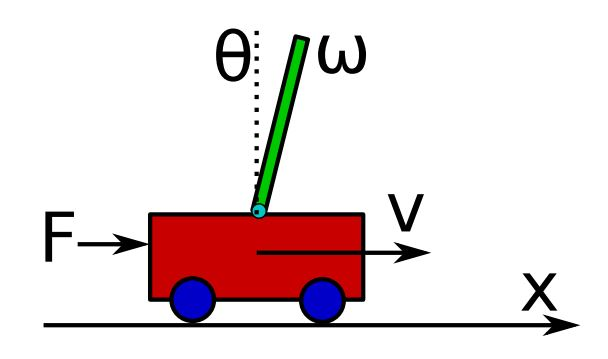
\includegraphics[width=0.5\textwidth]{Immagini/CartPole.JPG}
	\caption{Cart pole e variabili di stato}
	\label{fig:CartPole}
\end{figure}

Il pendolo inverso rappresenta un classico problema relativo alla \textit{dinamica} e alla \textit{teoria del controllo} ed è spesso utilizzato come \textit{problema dummy} per verificare e testare alcune strategie di controllo.
Si capisce quindi che, per mantenere il pendolo inverso nella posizione di equilibrio instabile, risulta essere necessario andare ad applicare una coppia sul punto di giunzione tra l'asta e il carrello, andando a muovere orizzontalmente a destra e a sinistra il carrello.
\section{RL e controllo}
Questo problema trova quindi una forte applicazione, come già sottolineato, nell'ambito della teoria del controllo: ma quindi, come possiamo applicare tecniche di reinforcement learning per andare a completare questo compito, ovvero quello di cercare di mantenere il pendolo in posizione verticale?

Come ben sappiamo, e come è evidente nel contesto del Cart Pole (figura ~\ref{fig:ActionBehaviour}), si tratta di andare a determinare il corretto input (\textit{azione}) al sistema il quale genererà il comportamento desiderato.

\begin{figure}[!h]
	\centering
	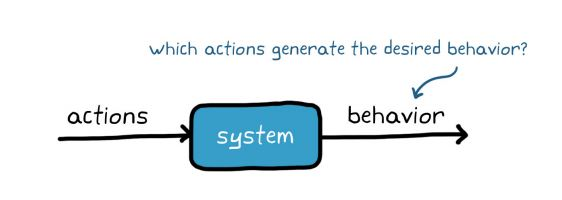
\includegraphics[width=0.4\textwidth]{Immagini/In_Out.JPG}
	\caption{Concetto di input-output}
	\label{fig:ActionBehaviour}
\end{figure}

La scelta dell'azione da portare all'ingresso del sistema, ovvero di quale movimento il carrello deve effettuare, solitamente viene realizzata andando ad utilizzare un sistema di retroazione ad anello chiuso, per cercare così di migliorare le prestazioni, riducendo l'errore (figura ~\ref{fig:ControlTheory})

\begin{figure}[!h]
	\centering
	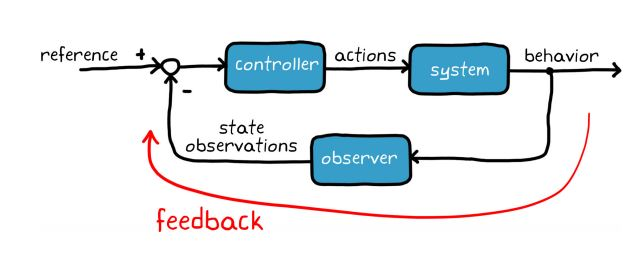
\includegraphics[width=0.6\textwidth]{Immagini/ControlTheory.JPG}
	\caption{Rete di retroazione}
	\label{fig:ControlTheory}
\end{figure}
Questo concetto è semplice da esprimere a parole e a livello grafico, però, nelle applicazioni reali, può diventare estremamente difficile da ottenere, nel momento in cui il sistema è molto complesso da modellizzare matematicamente, oppure presenta forti componenti non lineari, oppure ancora presenta un elevato spazio degli stati.

Ci viene quindi in aiuto, nel contesto del controllo, il reinforcement learning, il quale permette di andare a condensare in un'unica \textit{black-box} tutto il sistema di controllo, andando a ricevere come ingresso l'insieme di tutte le osservazioni dell'ambiente esterno e fornendo come output le azioni dirette (figura ~\ref{fig:SqueezingOfControlTheory})

\begin{figure}[h!]
	\centering
	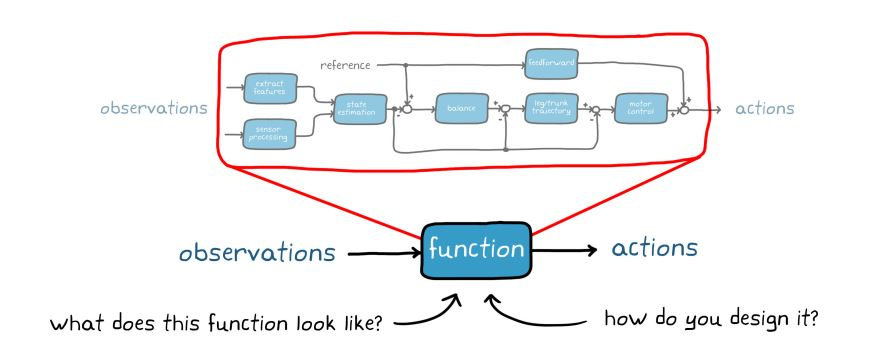
\includegraphics[width=0.8\textwidth]{Immagini/SqueezingOfControlTheory.JPG}
	\caption{Modellizzazione \textit{black - box}}
	\label{fig:SqueezingOfControlTheory}
\end{figure}

La peculiarità dei sistemi di reinforcement learning, a differenza delle altre due branchie del \textit{machine learning} (\textit{supervised learning e unsupervised learning}), sta nel fatto che essi vanno a lavorare con dati provenienti da ambienti dinamici, imponendosi l'obbiettivo di andare a trovare la miglior sequenza di azioni che andrà a generare il miglior \textit{output}, ovvero vale a dire il più alto reward ottenibile dall'agente stesso.

Nel fare questo l'agente risulta essere in grado di osservare lo stato attuale dell'\textit{environment}, decidendo poi quali azioni compiere: ovviamente, andando ad eseguire certe azioni, lo stato dell'ambiente cambia, fornendo un certo \textit{reward} all'agente stesso, in base al quale esso può valutare se l'azione eseguita era "buona" oppure se è meglio evitare di ripeterla (questo ciclo è sinteticamente rappresentato in figura ~\ref{fig:State_Action_Reward}).

\begin{figure}[h]
	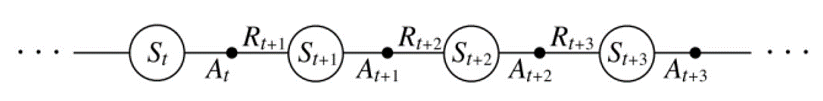
\includegraphics[width=0.7\textwidth]{Immagini/State_Action_Reward.png}
	\caption{Sequenza \textit{State-Action-Reward}}
	\label{fig:State_Action_Reward}
\end{figure}

In particolare, la da parte dell'agente di quale azione eseguire, in seguito a quello che è lo stato osservato, avviene per mezzo di una funzione la quale, nella nomenclatura del RL è chiamata \textit{policy} (figura ~\ref{fig:Policy}).

\begin{figure}[!h]
	\centering
	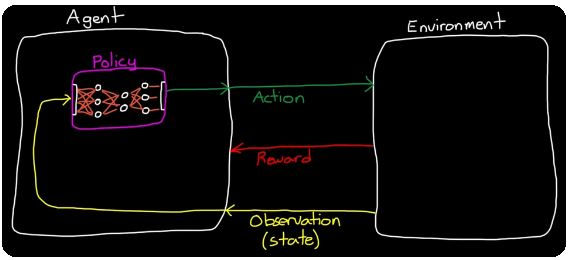
\includegraphics[width=0.7\textwidth]{Immagini/Policy.JPG}
	\caption{Policy}
	\label{fig:Policy}
\end{figure}

Ovviamente questa mappatura \textit{observation (state) - action} non può essere realizzata in maniera statica, anche se trovassimo la miglior policy: questo perchè l'ambiente potrebbe cambiare (e quasi sicuramente lo farà!) nel corso del tempo, e quindi una mappatura statica non sarebbe del tutto ottimale.

Questo quindi porta alla necessità di introdurre \textit{RL alogorithms}, i quali permettono di andare ad aggiornare la policy, in base alla stato-azione-reward, cercando quindi di scegliere la policy ottimale per ogni stato dell'ambiente., ovvero cercando di settare nella maniera migliore i parametri che caratterizzano la funzione espressa, in maniera generica, in figura ~\ref{fig:PolicyFunction}

\begin{figure}[!h]
	\centering
	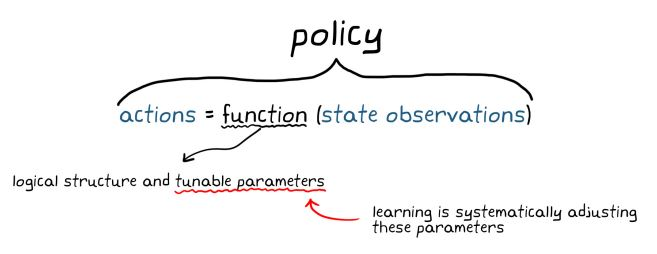
\includegraphics[width=0.5\textwidth]{Immagini/PolicyLearning.JPG}
	\caption{Significato di \textit{imparare} per un agente}
	\label{fig:PolicyFunction}
\end{figure}

\newpage

In sostanza questo update della policy può avvenire seguendo differenti algoritmi, come vedremo successivamente: in ogni caso, indipendentemente dalla strategia che si decide di seguire per scegliere l'azione successiva, possiamo modellizzare questo update come un blocco interno all'agente e che lavora direttamente sulla policy, basandosi sulla condizione attuale dell'ambiente, sull'azione che si va ad eseguire e sul reward che si ottiene eseguendola (il tutto è schemattizzato in figura ~\ref{label})

\begin{figure}[!h]
	\centering
	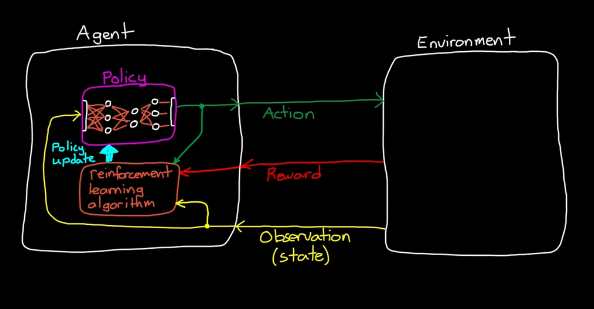
\includegraphics[width=0.5\textwidth]{Immagini/Policy_update.png}
	\caption{Policy update con algoritmi di \textit{RL}}
	\label{fig:Policy_update}
\end{figure}


E' a questo punto che possiamo quindi esplicitare il diretto legame tra RL e control theory: come abbiamo visto con entrambi i metodi vogliamo andare a determinare la corretta azione da eseguire sul sistema, per ottenere il comportamento desiderato, da cui si ricava il feedback, che corrisponde alle osservazioni dello stato del sistema (figura ~\ref{fig:RL_Control}).

\begin{figure}[!h]
	\centering
	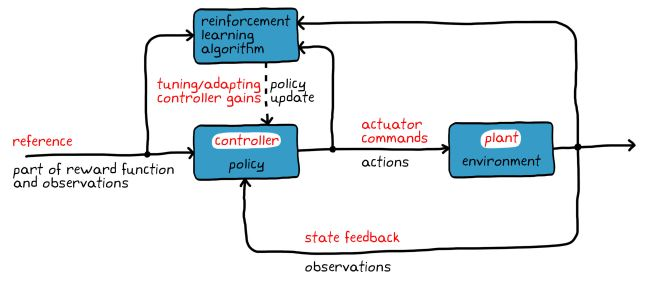
\includegraphics[width=0.7\textwidth]{Immagini/RL_Control.JPG}
	\caption{RL inteso come \textit{control theory}}
	\label{fig:RL_Control}
\end{figure}
\section{Cart Pole environments and reward}
s
Come già esplicitato in precedenza l'obbiettivo del problema legato al \textit{cart-pole} è quello di andare a bilanciare l'asta applicando una forza orizzontale al carrello. 

L'aspetto principale da considerare è quello relativo allo spazio degli stati: esso rappresenta cosa l'agente va ad osservare del sistema, e quindi quali variabili andrà ad utilizzare per controllare il sistema stesso. Nel nostro caso, e nel caso genrico di studio del cart pole, le variabili di stato utilizzate sono:
\begin{itemize}
	\item \textbf{Posizione del carrello (x)};
	\item \textbf{Velocità del carrello (\textit{v})};
	\item \textbf{Angolo di inclinazione della barra ($\theta$)};
	\item \textbf{Velocità angolare della barra ($\omega$)};
\end{itemize}

L'asta è considerata bilanciata in maniera corretta se entrambi le seguenti condizioni sono rispettate:
\begin{itemize}
	\item l'angolo dell'asta rimane compreso in un range attorrno alla posizione verticale (la quale corrisponde a 0 \textit{rad});
	\item la posizione del carrello rimane all'interno di uno specifico intervallo.
\end{itemize}
Se una di queste due condizioni risulta essere invalidata, l'episodio specifico termina, facendo ripartire il training. Un'altra possibile via che conduce l'episodio verso la sua terminazione è quello in cui il reward dell'episodio in esame risulta essere superiore ad una certa soglia stabilita in maniera statica, il chè corrisponde a verificare che il carrello sia in grado di bilanciare l'asta per più di un certo numero di azioni (ovvero che ha effettivamente imparato a risolvere il problema che gli è stato sottoposto).

Possiamo individuare inoltre due possibili varianti dell'ambiente legato al problema del cart-pole, le quali differiscono per lo spazio degli stati dell'agente:
\begin{itemize}
	\item \textbf{Discreto:} l'agente può applicare al carrello una forza che può valere \textbf{$F_{max}$} oppure \textbf{$-F_{max}$}, che è rappresentata dalla proprietà \textit{MaxForce} all'interno del codice. In sostanza ciò consiste nell'avere solo due azioni, le quali all'interno del codice sono identificate con due differenti numerazioni. Per esempio, la classica scelta, può essere quella di andare ad assegnare
	\begin{itemize}
		\item  \textbf{0} per l'azione di spinta del carrello verso sinistra;
		\item  \textbf{1} invere se l'agente vuole muoversi verso destra.
	\end{itemize}
	\item \textbf{Continuo:} l'agente può applicare una forza che varia in maniera continua all'interno dell'intervallo $[-F_{max}, F_{max}]$.
\end{itemize}

Un altro aspetto importante da definire è la tipologia di reward che l'ambiente ritorna all'agente: si possono operare diverse scelte. Un'opzione comunemente seguita, la quale sarà sfruttata anche all'interno di questo progetto, è quello di andare a ad \textbf{incrementare il reward di una unita} ad ogni iterazione all'interno di un episodio, fintantochè esso non termina. 

Quindi, più l'episodio si protrae nel tempo, più l'agente mantiene in equilibrio l'asta e, di conseguenza, più reward otterrà.


\chapter{Implementazione}
\section{Algoritmo Q learning}
\subsection{Perchè Q-learning?}
E' importante sottolineare come, nella letteratura relativa all'ambito del reinforcement learning, si è soliti andare a lavorare con quattro funzioni, che permettono di specificare come l'agente cambia la propria policy in funzione dell'esperienza acquisita, come si vede nella figura ~\ref{fig:Policy_update}.
Ovviamente, l'obbiettivo dell'agente è quello di ottenere il reward massimo fintantoche continua ad eseguire l'azione per cui è stato concepito: potremmo quindi introdurre il concetto di \textit{discounted return} al tempo \textit{t} definibile come:

\begin{center}
	$G_t = R_{t+1} + \gamma R_{t+2}+ \gamma^2\bullet R_{t+3} + ...$
	\label{eq:discounted_return}
\end{center}

dove con il coefficiente $\gamma$ andiamo a definire la \textit{lungimiranza} dell'agente: infatti se $\gamma = 0$ l'agente risulta essere \textit{greedy}, cercando di massimizzare il reward immediato; invece, mantenendo $\gamma < 1$, l'agente risulta essere in grado di dare un peso più o meno maggiore ai reward successivi, garantendo comunque la convergenza della sommatoria ~\ref{eq:discounted_return}.

Questa funzione appena introdotta risulta essere necessaria per definire due funzioni molto importanti:
\begin{itemize}
	\item \textbf{Value of a state, given a policy: } $v_\pi(s)$ che rappresenta il reward totale che ci si aspetta se l'agente segue la policy $\pi$ dall'istante t fino a $\infty$;
	\item \textbf{Value of a state-action pair, given a policy: } $q_\pi(s,a)$ indica sempre il reward che cumulerò seguendo sempre la stessa policy $\pi$, dopo però aver eseguito, nell'istante $t$ una specifica azione $a$.
\end{itemize}

I valori ottimali di queste funzioni, per completezza, sono rappresentati con l'apice $^*$, mentre i valori stimati, che sono quelli con cui poi si va effettivamente a lavorare, sono indicati tramite le lettere maiuscole, come si può notare nella figura ~\ref{fig:ValueFunctions}.

\begin{figure}[!h]
	\centering
	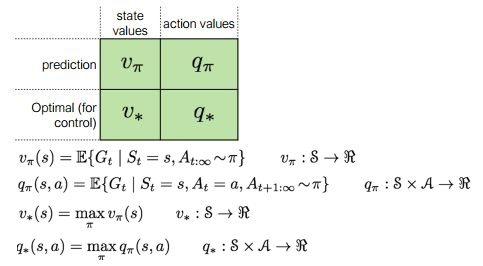
\includegraphics[width=0.5\textwidth]{Immagini/4_valueFunctions.JPG}
	\caption{4 value functions utilizzate per la policy update}
	\label{fig:ValueFunctions}
\end{figure}

Si può quindi facilmente intuire da dove deriva la nominazione di questo algoritmo: esso basa il proprio funzionamento sulla funzione \textit{Q}, la quale rappresenta la funzione cosidetta \textit{quality}, ovvero che indica quanto è utile una certa azione per aumentare il reward che si andrà ad ottenere nel futuro: si tratta inoltre di un algoritmo \textit{off-policy} poichè la funzione di q-learning apprende da azioni che stanno all'infuori delle policy corrente.
Essa può essere inserita in un quadro più generale di 4 funzioni, utilizzabili appunto dell'algoritmo di reinforcement learning per andare a gestire quella che è la policy dell'agente: esse sono riportate in figura ~\ref{fig:ValueFunctions}, con i rispettivi calcoli \textit{asintotici} necessari per ricavarne il valore.

Come evidenziato in precedenza, non possiamo però lavorare con i valori ottenibili tramite operatori di valore atteso, ma bensì risulta essere necessario andare ad utilizzare gli elementi stimati, ovvero rispettivamente $V_t(s)$ e $Q_t(s,a)$.

\subsection{Q-learning off policy control}
Il Q learning, come la maggior parte degli algoritmi di RL, va alla ricerca di un trade-off tra \textit{esploration e exploitation}: nel caso del Q learning si cerca, tramite un fattore di esplorazione (\textit{exploration rate}), di spingere l'algoritmo verso una scelta esplorativa piuttosto che di apprendimento, cercando di mantenere quindi una politica maggiormente esplorativa all'inizio del training per poi spostare l'attenzione sul fattore di apprendimento.
Il fatto che si tratti di un algoritmo off policy richiede in ingresso parametri aggiuntivi oltre a quelli forniti dall'ambiente (dimensione dello stato, numero di azioni...).
Tre sono i parametri aggiuntivi: $\alpha,\epsilon,\gamma$ che rappresentano rispettivamente 
\begin{itemize}
	\item learning rate: determina con quale estensione le nuove informazioni acquisite sovrascriveranno le vecchie informazioni; un fattore 0 impedirebbe all'agente di apprendere, al contrario un fattore 1 farebbe si che l'agente si interessi solo delle informazioni recenti
	\item exploration rate
	\item discounting rate: dovrebbe essere l'unico fattore non soggetto a decadimento, dato che esso determina l'importanza delle ricompense future, bilanciando reward immediato e futuro. Un fattore pari a 0 renderà l'agente opportunista, facendo si che consideri solo le ricompense attuali, mentre un fattore tendente ad 1 renderà l'agente attento anche alle ricompense che riceverà in futuro a lungo termine.
\end{itemize}
Per semplificare la trattazione, in questo contesto si è deciso di non considerare il decadimento dei parametri.

\begin{figure}[!h]
	\centering
	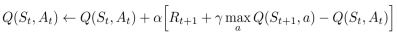
\includegraphics[width=0.5\textwidth]{Immagini/Q_estimation.JPG}
	\caption{Equazione di \textit{Bellman} utilizzata per andare ad aggiornare i valori della funzione Q}
	\label{fig:Q_estimation}
\end{figure}

Questa formula per l'update è stata implementata direttamente nel codice (come si vede in figura ~\ref{fig:Q_update}) all'interno dell'algoritmo ~\ref{alg:Q_policy}: in particolare è da evidenziare come il pedice $t$ applicato allo \textit{state} e \textit{action} rappresenta la condizione attuale; il pedice $t+1$ applicato allo stato, vuole invece rappresentare lo stato successivo che si raggiunge eseguendo l'azione A all'istante $t$.

\begin{figure}[!h]
	\centering
	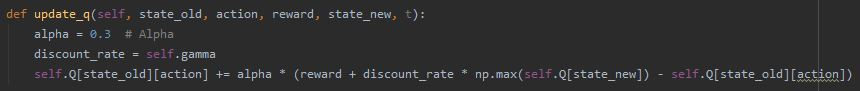
\includegraphics[width=0.5\textwidth]{Immagini/Q_update.JPG}
	\caption{Aggiornamento Q table}
	\label{fig:Q_update}
\end{figure}

\begin{algorithm}
		\SetAlgoLined
		\KwData{Parametri dell'algoritmo: step size $\alpha$ (con $0<=\alpha<=1$), $\epsilon>0$}
		\While{non sono terminati gli episodi:}{
			Inizializza lo stato S
			
			
			\While{non sono terminati gli step:}{
				Scegli azione A usando la policy derivata da Q (per esempio epsilon-greedy)
				
				
				Esegui l'azione A, osservando il reward (R) ottenuto e il nuovo stato (S') raggiunto
				
				
				Aggiorna Q(S,A) secondo la formula ~\ref{fig:Q_estimation}
				
				
				$S \leftarrow S'$ 
				
				
				Continua fino a che non si raggiunge uno stato terminare
			}
		}
		\caption{Q learning per la stima della policy $\pi$}
		\label{alg:Q_policy}
\end{algorithm}

\subsection{Scelta dell'azione e Q table}
Il metodo \textit{choose action} mostrato in figura ~\ref{fig:ChooseAction_Bucket}, permette la scelta dell'azione da intraprendere sulla base del trade off illustrato precedentemente tra esplorazione e apprendimento: si va infatti a scegliere la policy greedy che consiste in una scelta randomica dell'azione, oppure viene utilizzata la target policy a cui corrisponde il valore maggiore nella tabella stato-azione.
Si capisce quindi come Q-learning (in genere) sia in grado di andare a tener conto del problema di avere un trade-off tra:
\begin{itemize}
	\item \textbf{Exploiting: }scegliendo l'azione basata sul massimo valore della specifica azione, l'agente continua a rimanere fissato in quel punto, sfruttando al massimo il reward ottenibile, senza cercare eventuali altri stati in grado di fornire maggior reward;
	\item \textbf{Exploring: }selezionando randomicamente un'azione, rendiamo l'agente in grado di esplorare e scoprire nuovi stati, che altrimenti non avrebbe mai esplorato. 
\end{itemize}
\begin{figure}[!h]
	\centering
	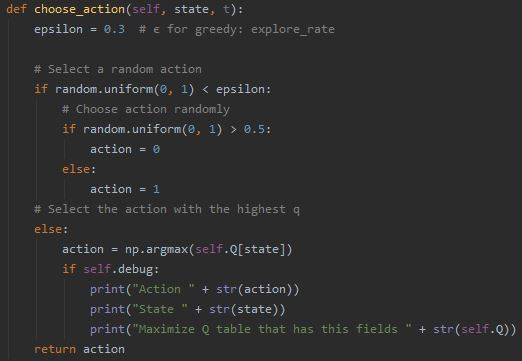
\includegraphics[width=0.5\textwidth]{Immagini/ChooseAction_QTable.JPG}
	\caption{Metodo per la stima della azione da eseguire}
	\label{fig:ChooseAction_Bucket}
\end{figure}

In particolare risulta quindi essere necessario spostarsi da uno spazio degli stati continuo ad uno discreto, con un numero finito e preferibilmente piccolo di stati discreti: infatti, meno stati abbiamo, più piccola risulterà essere la Q-table, e meno step l'agente dovrà eseguire per apprendere correttamente i valori che compongono la tabella. 

Tuttavia, pochi stati, potrebbero non essere sufficienti per rappresentare l'ambiente: nella nostra implementazione si è deciso di andare a discretizzare solamente 2 delle 4 variabili di stato, ovvero l'angolo $\theta$ e la velocità angolare $\theta'$ della barra; per quanto riguarda invece la posizione e la velocità del carrello, non discretizzandole, le si va a mappare come dei singoli valori scalari. La motivazione è il fatto che la probabilità del carrello di lasciare l'ambiente a destra o a sinistra e molto bassa, dando quindi maggior peso alla riduzione della dimensionalità.
Questa discretizzazione degli stati si traduce, a lato pratico, in una matrice con una struttura particolare, la quale dipende dal numero di bucket che si stanno utilizzando: supponiamo di aver settato, all'interno del nostro script Python, un vettore $buckets=(1, 1, 4, 5,)$: la Q-table risultante da questa discretizzazione è quella rappresentata in figura ~\ref{fig:Q_table_example} in cui si può vedere come, per ogni discretizzazione dell'angolo corrisponde un nuovo blocco di un numero di righe pari alla discretizzazione richiesta invece per la velcoità angolare. All'interno di ogni singola riga troviamo due differenti valori, i quali rappresentano appunto i Q-values relativi alle due possibili azioni eseguibili in ogni diverso stato.

\begin{figure}[!h]
	\centering
	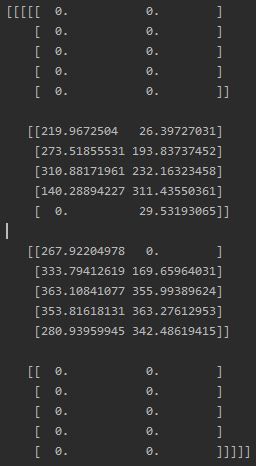
\includegraphics[width=0.2\textwidth]{Immagini/Example_of_Q_table.JPG}
	\caption{Possibile struttura della Q-table}
	\label{fig:Q_table_example}
\end{figure}

\subsection{Result}
La figura ~\ref{fig:QLearning_result} riportà l'andamento del reward in fase di training. L'algoritmo si considera risolto quando completa con successo 195 episodi consecutivi (sui 200 massimi disponibili): si nota infatti come nel grafico tutti gli ultimi total reward registrati siano sopra la soglia di vincita dell'algoritmo (linea verde).
L'andamento espresso dalla linea rossa invece indica un valore più \textit{smooth} del reward.

\begin{figure}[!h]
	\centering
	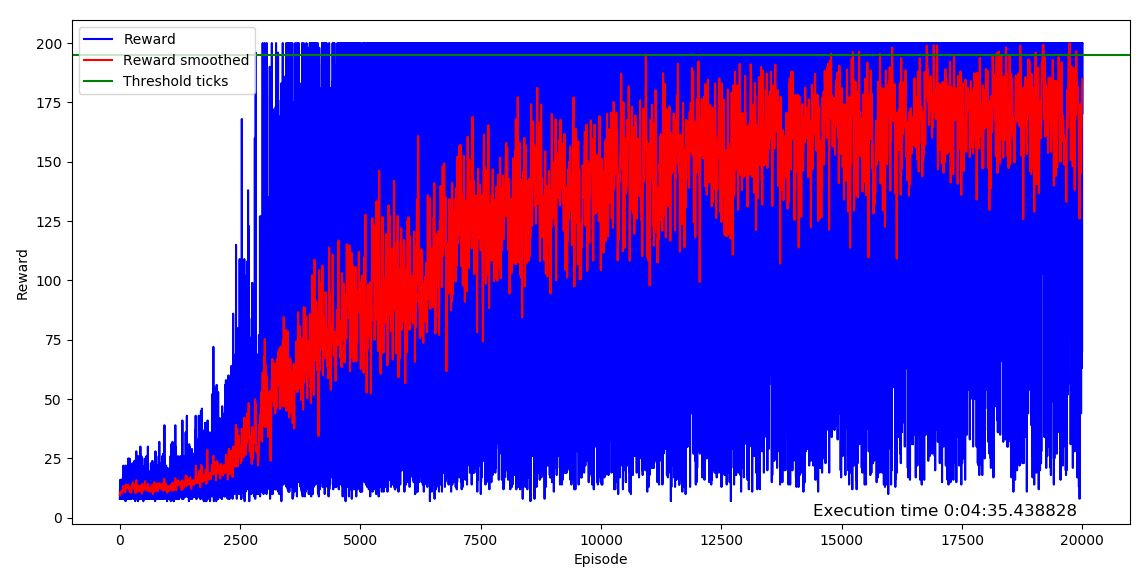
\includegraphics[width=0.8\textwidth]{Immagini/reward_20K.JPG}
	\caption{Andamento del Q learning}
	\label{fig:QLearning_result}
\end{figure}

Per andare a realizzare un confronto tra i diversi algoritmi, si è runnato l'agoritmo di Q-learning a bucket con un batch di 2000 iterazioni, ognuna delle  quali aveva una \textit{time threshold} di 200 iterazioni: come si può vedere in figura ~\ref{fig:QLearning_poor_result} il limite di iterazioni minime in cui il pole viene mantenuto in equilibrio non viene raggiunto. Si può notare anzi come l'agente non venga \textit{trainato} a sufficienza, raggiungendo prestazioni molto basse, rispetto ai successivi algoritmi.

\begin{figure}[!h]
	\centering
	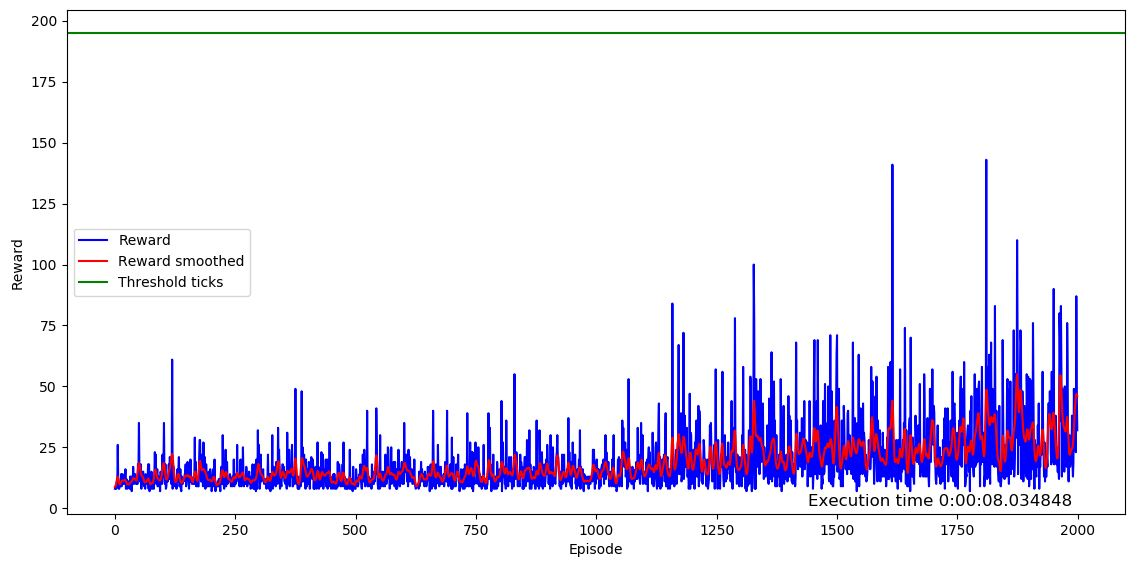
\includegraphics[width=0.8\textwidth]{Immagini/reward_2K.JPG}
	\caption{Andamento del Q learning confrontabile con atri algoritmi implementati}
	\label{fig:QLearning_poor_result}
\end{figure}

\newpage


\section{Algoritmo DQN}
La soluzione al problema di discretizzazione degli stati con conseguente perdita di informazioni che potrebbe risultare importanti e decisive al learning dell'ambiente, viene risolta grazie all'algoritmo di Deep Q-network: la Q-table viene infatti sostituita da una rete neurale, la quale non necessita più di alcuna forma di discretizzazione che approssima la funzione valore.

La rete prende come input lo stato e produce una stima della funzione valore per ogni azione: in particolare si tratta di una rete \textit{fully-connected}, in cui l'imput della network sono le quattro variabili di stato
\begin{itemize}
	\item Posizione (\textit{x})
	\item Velocità lineare ($\dot{x}$)
	\item Angolo ($\theta$)
	\item Velocità angolare ($\dot{\theta}$)
\end{itemize}
mentre le uscite rappresentano i Q-values per le due possibili azioni, ovvero il movimento a destra e a sinistra, come si può vedere in figura ~\ref{fig:DQN_network}.

\begin{figure}[!h]
	\centering
	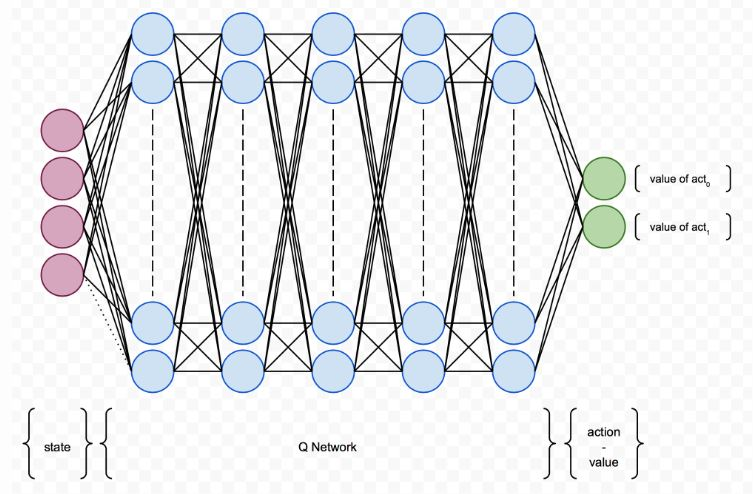
\includegraphics[width=0.5\textwidth]{Immagini/DQN_network.JPG}
	\caption{DQN network}
	\label{fig:DQN_network}
\end{figure}

\subsection{Q network}
Nell'implementazione, per andare a realizzare la rete neurale, è stata utilizzata la libreria python TensorFlow, basandosi sulle API fornite da Keras, per una facile creazione della rete neurale, in maniera molto rapida e concisa.

\begin{lstlisting}
	model = Sequential()
	model.add(Flatten(input_shape=(1,) + env.observation_space.shape))
	model.add(Dense(16))
	model.add(Activation('relu'))
	model.add(Dense(nb_actions))
	model.add(Activation('linear'))
\end{lstlisting}

Tramite l'utilizzo di una rete neurale quindi, andiamo a sostituire l'update della Q table, con il train della nostra rete neurale: come infatti ben sappiamo, il modello \textit{DQN neural network} è un modello di regressione, il cui output è tipicamente un valore continuo (\textit{float value}, che rappresenta direttamente valore della nostra Q function. L'agente, come sempre, andrà a scegliere l'azione che presenta il Q-value maggiore, che indica appunto quale è l'azione che si presume che andrà a dare un maggiore reward nel futuro.

\begin{figure}[!h]
	\centering
	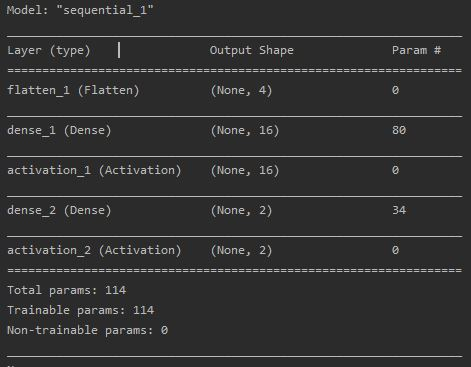
\includegraphics[width=0.5\textwidth]{Immagini/Model_of_my_net.JPG}
	\caption{Modello della rete neurale: 4 input \textit{state} e 2 output \textit{Q-action}}
	\label{fig:Model_of_DQN_network}
\end{figure} 


\subsection{Replay memory}
Introducendo una rete neurale, invece della Q-table utilizzata durante la prima versione del Q learning, la complessità del nostro ambiente può crescere significativamente, senza richiedere necessariamente più memoria: come si può facilmente vedere, un environment a celle con grandezza $50 \times 50$, andrebbe ad esaurire facilmente la memoria della maggior parte dei pc in commercio.
Invece, con una rete neurale, anche con ambienti complessi, non dobbiamo affrontare problemi legati ai requisiti di memoria
Per gestire questo utilizzo di memoria, un concetto da illustrare è quello dell’experience replay, codificato tramite il comando presentato in figura ~\ref{fig:SeqMem}.

\begin{figure}[!h]
	\centering
	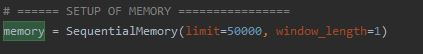
\includegraphics[width=0.5\textwidth]{Immagini/SequentialMemory.JPG}
	\caption{Creazione variabile per sequential memory}
	\label{fig:SeqMem}
\end{figure}

Gli algoritmi di reinforcement learning presentano infatti spesso il problema di avere un alto livello di correlazione tra esperienze successive con l'alto rischio di portare ad un veloce overfitting sui dati a disposizione, evitando così la necessaria generalizzazione.

L’idea della experience replay è quindi quella di salvare le esperienze
in una memoria chiamata replay memory e durante ogni passo di learning recuperare in maniera randomica un campione di tali transazioni, per andare così ad introdurre una forte incorrelazione tra misure sequenziali.
Questo è dimostrato come esso vada a stabilizzare e a migliorare la procedura di training della rete neurale DQN.

\subsection{Result}
\begin{figure}[!h]
	\centering
	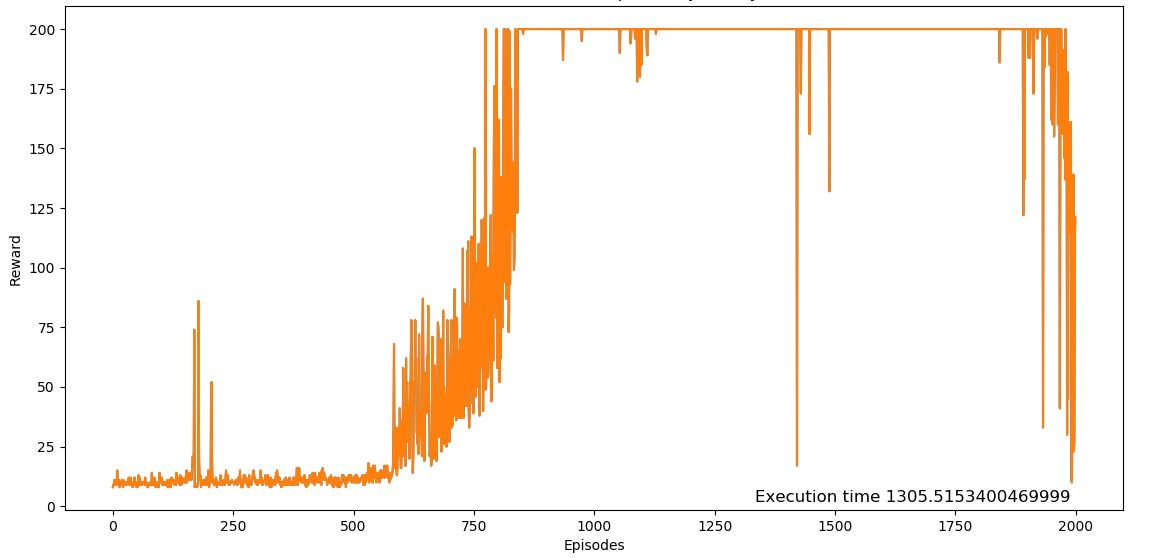
\includegraphics[width=\textwidth]{Immagini/DQN_Agent.JPG}
	\caption{Reward con DQN network}
	\label{fig:DQN_reward}
\end{figure}

\newpage
\section{Algoritmo \textit{Finite Differences}}
Negli algoritmi visti fin'ora, per trovare la policy adatta ($a = \pi(s)$ dove con $\pi$ indichiamo appunto la \textit{policy}) siamo sempre andati ad utilizzare una funzione approssimata $Q_{\pi^*}(s,a)$, la quale permetteva all'agente di scegliere quale fosse l'azione migliore da compiere, sia nel caso di azioni discrete, sia nel caso di azioni continue che discrete ()come si vede in figura ~\ref{fig:Q_function_utility}) andando poi a selezionare l'azione in grado di massimizzare l'output.

\begin{figure}[!h]
	\centering
	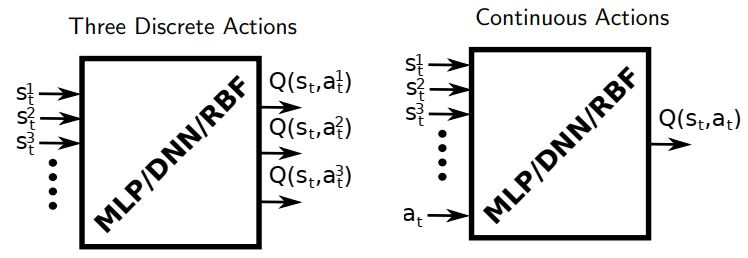
\includegraphics[width=0.8\textwidth]{Immagini/Q_function_utility.JPG}
	\caption{Valutazione della funzione sulla base della Q-values}
	\label{fig:Q_function_utility}
\end{figure}

La domanda che ci poniamo è: \textit{possiamo trovare la policy direttamente} partendo dallo stato attuale ($s_t$) e ottenendo appunto $a_t$?

La risposta è si.

\begin{figure}[!h]
	\centering
	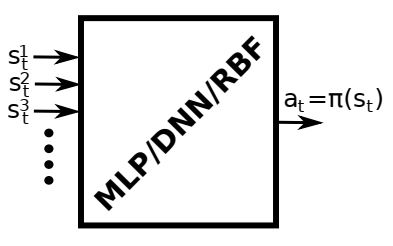
\includegraphics[width=0.5\textwidth]{Immagini/No_Q_function.JPG}
	\caption{Valutazione della funzione \textit{non} basandosi sulla Q-values}
	\label{fig:NO_Q_function_utility}
\end{figure}
Questo concetto, mostrato in maniera molto diretta nella figura ~\ref{fig:NO_Q_function_utility}, è quello che nella letteratura del RL viene chiamato come metodo di \textit{policy search}, il quale permette appunto di stimare la polici ottimale ($\pi^*(a|s)$) invece di cercare il valore ottimo per la funzione $Q^*(s,a))$: questo nuovo approccio presenta innumerevoli vantaggi rispetto agli algoritmi mostrati in precedenza, in particolare:
\begin{itemize}
	\item Policies ottimali, scelte tramite algoritmi di questo tipo, presentano un numero di parametri minore rispetto al valore ottimale della q-functions (\textit{curse of dimensionality})
	\item Processo di learn più veloce (e questo è anche dimostrato dai grafici presenti all'interno di questa documentazione)
	\item Offre la possibilità di utilizzare policies sia deterministiche che stocastiche (\textit{noisly})
\end{itemize}

\textit{E cosa cerchiamo di ottimizzare in questo nuovo contesto?}
I metodi di policy search vanno ad ottimizzare l'indice $J(\theta)$, dove $\theta$ rappresenta il vettore dei pesi; è possibile realizzare questa ottimizzazione utilizzando differenti metodi:
\begin{itemize}
	\item Gradient free methods:
	\begin{itemize}
		\item Evolutionary computation
		\item Simulated annealing
		\item Hill climbing
	\end{itemize}
	\item \textbf{Gradient based methods} (\textit{policy gradient methods}):
	\begin{itemize}
		\item  Gradient estimation 
		\item Optimization algorithm
	\end{itemize}
\end{itemize}

I passi principali che sono stati implementati, sono
\begin{itemize}
	\item Implementare la dinamica del carrello (di cui non si riporta la trattazione) e una funzione per simulare i roll-outs (sotto sezione ~\ref{sec:rollout}) che forniscono il reward di ritorno;
	\item Utilizzare una \textit{Radial Basis Function} (RBF network - sotto sezione ~\ref{sec:RBF}) per approssimare l'apprendimento, ovvero per ottenere $a = \pi(s,W) = W^T\Phi(s,a)$
	\item Implementare l'algoritmo alla differenze finite (FD) per apprendere i pesi della policy
\end{itemize}

\subsection{Approccio \textit{Policy gradient estimation}}
Come già sottolineato in precedenza andremo a basarci su un algoritmo \textit{gradient based}, nello specifico l'agoritmo alla differenze finite, il quale, in ambito matematico, rappresenta una strategia utilizzata per risolvere numericamente equazioni differenziali che si basa sull'approssimazione delle derivate con equazioni alle differenze finite.

Questa approssimazione che andiamo ad utilizzare per effettuare un'operazione di minimizzazione (anche locale) sulla funzione $J(\theta) = V_\pi(s)$ \label{eq:J_function_to_minimize}: l'approccio che si è deciso di seguire non è però quello classico, ma bensì una strada alternativa, in cui, fornita una policy parametrizzata $\pi(a|s,\theta)$, possiamo calcolare $J(\theta)$ simulando l'environment come un \textit{Markov Decision Process}, la funzione $J(\theta)$. 

In particolare:
\begin{itemize}
	\item Invece di calcolare $\partial V / \partial\phi_i$ separatamente (passaggio che verrebbe naturale dopo aver definito $J(\theta)$ in \ref{eq:J_function_to_minimize}), andiamo ad ottenere un vettore random $\delta ~ N (0, \sigma^2)$.
	Nel codice questa parte è stata implementata in questo modo:
	\begin{lstlisting}
	# Variance of the random Gaussian perturbation of the parameters
	variance_of_perturbation = 0.1 
	# random parameter 	variation (Gaussian)
	delta = variance_of_perturbation * np.random.randn(numberOfCentrum, 1) 
	\end{lstlisting}
	\item Il vettore randomico generato in precedenza lo utilizzeremo poi per calcolare, tramite la tecnica definita \textit{roll-out} (sezione ~\ref{sec:rollout}), due valori della funzione J ($J_+, J_-$)
	\item Utilizzando l'approssimazione di taylor possiamo scrivere $J_+ \approx J(\Theta) + \nabla J^T \delta$ e $J_- \approx J(\Theta) - \nabla J^T \delta$
	\item La differenza $J_\Delta = J_+ - J_-$ diventa $J_\Delta = 2 \delta^T \nabla J$, dove $J_\Delta$ è un numero scalare mentre $\nabla J$ e $\delta$ sono vettori.
\end{itemize}

Questo processo andiamo a ripeterlo più volte con differenti valori randomici di $\delta_i$ con $i= 1,2,...N_H$: andremo quindi ad ottenere così differenti $J_{\Delta_i}$, ma ci sarà solamente un gradiente ($\nabla J$ sconosciuto).

In forma matriciale quindi diventa:
\begin{figure}[h!]
	\centering
	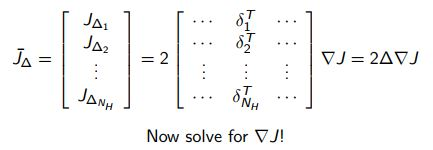
\includegraphics[width=0.7\textwidth]{Immagini/Matrix_form.JPG}
	\caption{Matrix form}
	\label{fig:matrix_form}
\end{figure}
La soluzione dovrebbe essere data da $\nabla J = 1/2 \Delta^{-1} J_\Delta$, ma $\Delta$
potrebbe non essere una matrice quadrata (per il fatto che il numero di rollout potrebbe non essere pari alla dimensione di $\Theta$): con alcuni passaggi matematici (qui omessi) possiamo andare una forma più stabile per ricavare la soluzione (riportata anche in precedenza) data da $\Delta J = 1/2 [\Delta^T \Delta +\lambda I]^{-1} \Delta^T J_\Delta$
\newpage
\subsection{Algoritmo \textit{FD}}
Questo è l'algoritmo implementato nel codice per apprendere i parametri ottimi. 
La corrispondeza implementata in \textit{Python} dell'algoritmo ~\ref{alg:FD_alg} la si trova nella figura ~\ref{fig:FD_py_alg}.

\begin{algorithm} [h!]
	\SetAlgoLined
	\caption{Finite Differences algorithm}
	\label{alg:FD_alg}
	\KwIn{Input: approssimazione della funzione parametrica $\pi(\bullet,\bullet,\Theta)$}
	\KwOut{Output: pesi ottimali $\Theta^*$}
	\KwData{Parametri: \textit{Learning rate $\alpha$}, $\lambda$, $\sigma_\delta ^2$, numero di rollout}
	\While{Policy non converge}{
		Inizializza $J_\Delta$ e $\Delta$
		
		\For{$i = 1,2,..., N_H$}{
			Inizializza lo stato iniziale $s_0$
			
			Genera una variazione randomica $\delta$ distribuita come $N(0,\sigma_\delta^2)$
			
			$J_+ \leftarrow rollout(\pi(\Theta + \delta))$
			
			$J_- \leftarrow rollout(\pi(\Theta - \delta))$
			
			Add $J_+ - J_-$ al parametro  $J_\Delta$
			
			Add $\delta^T$ a $\Delta$
		}
		$\Theta^* \leftarrow \Theta^* + 1/2\alpha [\Delta^T \Delta + \lambda I]^{-1} \Delta^T J_\Delta$
	}
\end{algorithm}

\begin{figure}[!h]
	\centering
	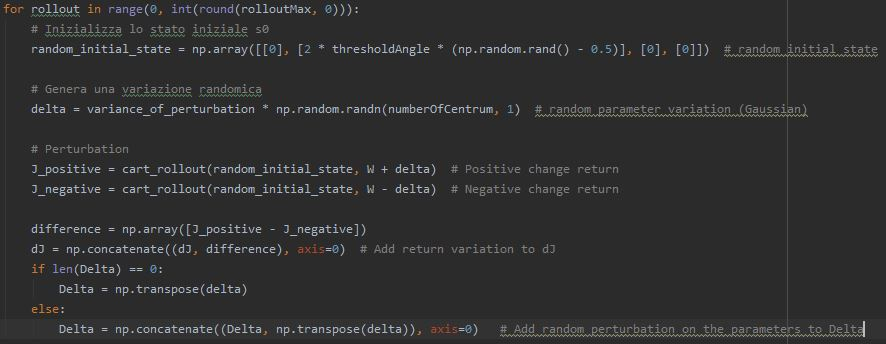
\includegraphics[width=\textwidth]{Immagini/FD_alg_python.JPG}
	\caption{Reward \textit{Finite Differences in Python}}
	\label{fig:FD_py_alg}
\end{figure}

\subsubsection{Rollout}
\label{sec:rollout}
Fornita una policy $a = \pi(s)$ oppure $a = \pi(a|s)$ e uno stato iniziale $s_0$ ad un certo istante temporale di un \textit{Markov Decision Process}, un rollout (definibile anche come \textit{traiettoria, storia o trial}), è semplicemente una sequenza \textbf{$H = s_0, a_0, s_1, a_1, .. , s_T, a_T$} generata a partire da uno stato $s_0$ e seguendo una policy $\pi$.
Nella implementazione relativa a questo progetto, come spiegato nella sotto sezione ~\ref{sec:RBF}, siamo andati ad utilizzare come approssimazione della policy da seguire il risultato fornito in uscita da una \textit{Radial Basis Function} neural network. 

\begin{figure}[!h]
	\centering
	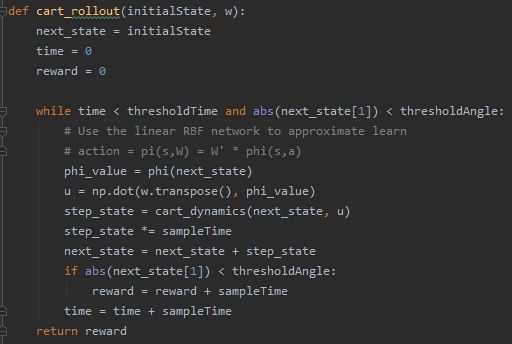
\includegraphics[width=0.7\textwidth]{Immagini/Rollout.JPG}
	\caption{Rollout in Python}
	\label{fig:roll_py}
\end{figure}

I pesi di questa rete neurale, come si può vedere nell'implementazione in figura ~\ref{fig:roll_py}, risultano però essere fissati, il che quindi equivale all'andare a seguire sempre la stessa policy.
\subsubsection{RBF network}
\label{sec:RBF}
Come è stato evidenziato in precedenza, siamo andati ad utilizzare una \textit{RBF} lineare per andare ad approssimare l'apprendimento.

In particolar modo le \textit{Radial Basis Function} permettono di andare a partizionare lo spazio degli stati, sovrapponendo dei \textit{"Gaussian neurons"}, in cui ogni neurone genera un segnale corrispondente al vettore di input: il segnale prodotto da ogni neurone presenta una potenza che dipende dalla distanza tra il centro della curva gaussiana che rappresenta il vettore e il vettore degli stati in input.

Questo concetto base delle \textit{RBF} viene implementato andando a creare una tabella formata da una sequenza di punti cartesiani, i quali rappresentano i centri di ognuno dei neuroni della rete neurale, ovvero la media di ogni curva gaussiana (figura ~\ref{fig:RBF_Centrum}).

\begin{figure}[!h]
	\centering
	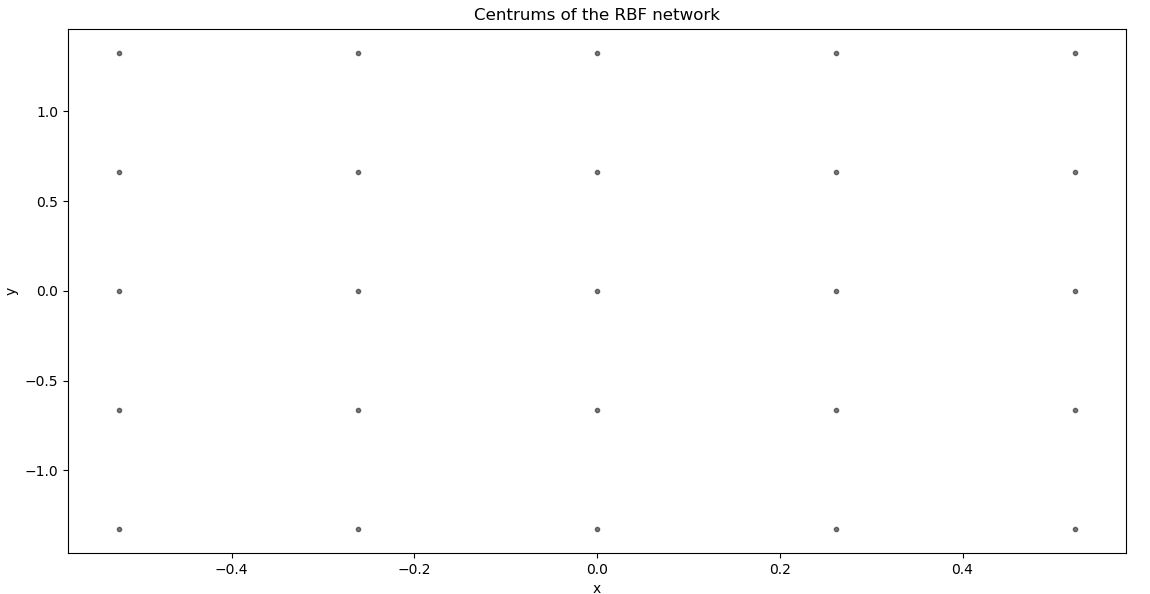
\includegraphics[width=0.5\textwidth]{Immagini/Centrum_of_RBF.JPG}
	\caption{Centri di ogni neurone della \textit{RBF}}
	\label{fig:RBF_Centrum}
\end{figure}

Un altro aspetto importante da evidenziare è il fatto che, i \textit{weigths} relativi alla \textit{RBF} vengono aggiornati tramite algoritmo Finite Difference: quindi, i

\subsection{Result}
Nella figura ~\ref{fig:Reward_FD}, è rappresentato l'andamento del reward con un batch di 10 trial con 70 iterazioni ciascuno: ogni iterazione può essere eseguita per un massimo di 10 s, nel caso in cui l'esecuzione non fallisce prima (ovvero il pole cade fuori dal range angolare imposto).
Si nota quindi come siano necessarie meno iterazioni, rispetto agli algoritmi precedenti, per ottenere un reward molto buono.

\begin{figure}[!h]
	\centering
	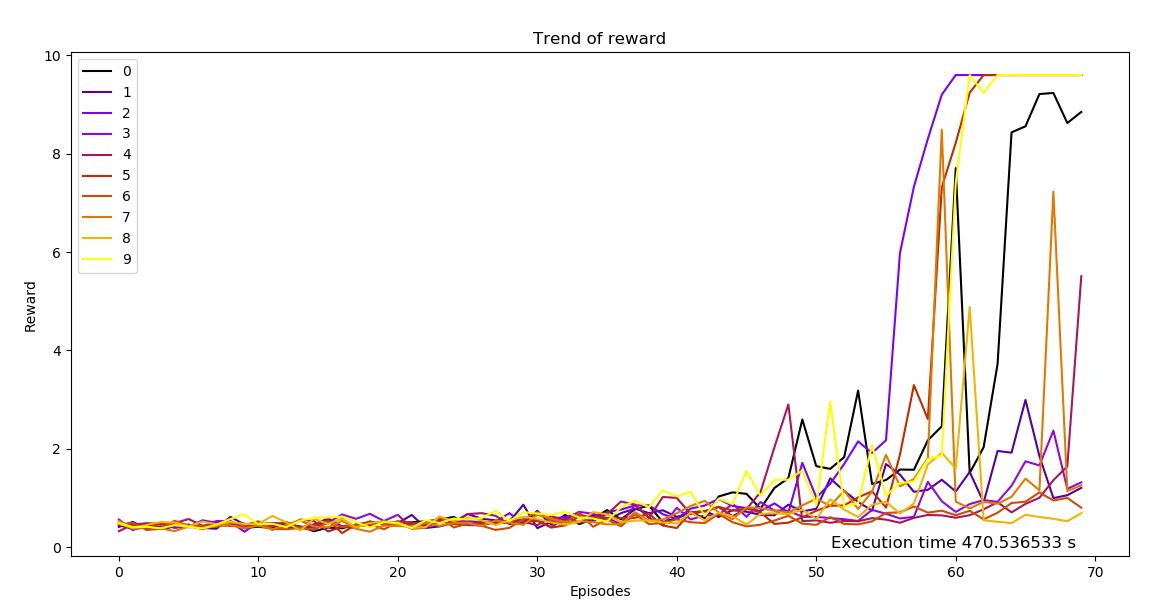
\includegraphics[width=\textwidth]{Immagini/Reward_FD.JPG}
	\caption{Reward \textit{Finite Differences}}
	\label{fig:Reward_FD}
\end{figure}

\newpage
\end{document}
